
 \chapter{\IfLanguageName{dutch}{Resultaten}{Resultaten}}
\label{ch:Resultaten}
In dit hoofdstuk zullen de resultaten van de testen en de enquête verwerkt worden om zo tot een antwoord te komen op dit onderzoek. Hierbij zijn de resultaten van de Cisco Identity Services Engine omgeving opgedeeld in 'Port-based en Policy-based network access control' en 'Tread-Centric en Policy-based network access control'. Vervolgens zijn de enquête resultaten verwerkt met een aantal grafieken waarbij dit terug te vinden is in Bijlage \ref{ch:Resultaten_enquête}. Meer informatie over de resultaten van de enquête vindt men in sectie \ref{sec:enqueteISe}.

\section{Cisco Identity Services Engine omgeving}
Zoals men ziet wordt Policy-based network access control steeds gecombineerd met Port-based en Thead-Centric network access control. Dit heeft als rede dat voor zowel Port-based, als voor Thread-Centric network access control, policy rules zijn toegepast.

\subsection{Port-based en Policy-based network access control}
Wanneer de use cases 'Port-based en Policy-based network access control' niet worden toegepast, dan kunnen gebruikers zich aansluiten op het netwerk zonder enige beveiliging. Dit is natuurlijk enkel mogelijk wanneer alle interfaces op het netwerk apparaat ingesteld zijn met het correcte vlan id. Anderzijds is het duidelijk dat eind apparaten zich eenvoudiger kunnen aansluiten op het netwerk zonder 'Port-based en Policy-based network access control'.
Als men de resultaten van de implemenatie van 'Port-based en Policy-based network access control' er bij halen, dan ziet men een duidelijk verschil in beveiliging ten opzichte van een netwerk zonder de use cases. Dit verschil is duidelijk te merken wanneer een gebruiker zich probeert aan te melden op het netwerk via één van de interfaces op de fysieke Cisco switch. Het eind apparaat krijgt een toegewezen ip adres van de vorm 169.254.x.x dat geen enkel compartiment van het netwerk kan bereiken. 
\newline
\newline
Het is echter wanneer de 'Wired AutoConfig' services aanstaan, kan men zich aanmelden op het netwerk door volgende stappen uit te voeren: 

\begin{itemize}
	\item Open het configuratiescherm, en ga naar 'netwerk en internet'.
	\item Open vervolgens het 'netwerkcentrum'.
	\item Open 'Adapter instellingen wijzigen'.
	\item Open het 'properties' tablad, door een rechtermuisklik op de correcte "Ehternet adapter".
	\item Vervolgens verschijnt het tablad "Authenticatie".
	\item Open "Extra instellingen".
	\item Veranderd het de 'authentication modus' naar gebruikers authenticatie.
\end{itemize}
Als de eind gebruikers de juiste gebruikersnaam en wachtwoord ingeeft, wordt de gebruiker met zijn apparaat aangesloten op het netwerk. Belangrijk om te weten is dat er een policy rule is ingesteld is dat alleen gebruikers van de groep 'Employees' toegang krijgen tot het netwerk. Het gebruik van de policy werd al eerder vernoemd in het hoofdstuk \ref{ch:Proof of concept}.
\newline
\newline
Figuur \ref{fig:Test_gebruiker} toont aan dat wanneer men wenst in te loggen met de gebruikersnaam 'Test' geen toegang krijgt tot het netwerk. Gebruiker 'Test' bevindt zich niet in de groep 'Employees' en zal dus als gevolg geen toegang krijgen tot het netwerk. Door het gebruik van policy rules wordt dankzij de test aangetoond dat policy rules ook de vruchten kan plukken op beveiliging.

\begin{figure}[H]
	\centering
	\subfloat{{\includegraphics[width=6.5cm]{Test_no_employee.png} }}%
	\qquad
	\subfloat{{\includegraphics[width=6.5cm]{Test_no_successed.png} }}%
	\newline
	\qquad
	\subfloat{{\includegraphics[width=14cm]{TestDenied.png} }}%
	\caption{Proef resultaat met een niet employee gebruiker}%
	\label{fig:Test_gebruiker}%
\end{figure}
	
Als men inlogt met een gebruiker die in de Cisco Identity Services Engine groep 'Employees' bevindt dan zal de gebruiker zonder problemen zich kunnen aansluiten op het netwerk. Dit wordt aangetoond in figuur \ref{fig:Test_gebruiker} waarbij een proef met de gebruiker 'TestV2' wordt uitgevoerd. Gebruiker 'TestV2' bevindt zich in groep 'Employees' waardoor het vanzelfsprekend is dat 'TestV2' met zijn eind apparaat met het netwerk kan verbinden. 

\begin{figure}[H]
	\centering
	\subfloat{{\includegraphics[width=6cm]{TestV2_Employee.png} }}%
	\qquad
	\subfloat{{\includegraphics[width=6cm]{TestV2_succeeded.png} }}%
	\newline
	\qquad
	\subfloat{{\includegraphics[width=13cm]{TestV2_succeeded_ISE.png} }}%
	\caption{Proef resultaat met een employee gebruiker}%
	\label{fig:Test_gebruiker}%
\end{figure}

Hierdoor kent Cisco Idendity Services Engine met use cases 'Port-based en Policy-based network access control' een positieve resultaat in een netwerk. In de sectie \ref{sec:trepo} worden de resultaten van Tread-Centric en Policy-based network access control besproken. Voor meer uitleg over de volledige conclusie kunt u terecht in Hoofdstuk \ref{ch:conclusie}.


\subsection{Tread-Centric en Policy-based network access control}
\label{sec:trepo}

\section{Cisco Identity Services Engine enquête}
\label{sec:enqueteISe}
In deze sectie worden de resultaten van de enquête globaal besproken. Indien men meer informatie wenst over de resultaten per vraag kan men Bijlage \ref{ch:Resultaten_enquête} raadplegen.
\newline
\newline
Bovenal mag men tevreden zijn met de responsen van de enquête daarnevens kent de enquête 14 responsen op 2 weken tijd. Helaas beschikt men niet over het grote netwerk om de responsen van de enquête te doen verhogen. Een groter aantal responsen zou resulteren in een veel nauwkeuriger resultaat.  
\newline
\newline
78.6\% van de geënquêteerden is gekend met het Cisco Identity Services Engine product. De ovigere 21.4\% is niet gekend met het Cisco Identity Services Engine product en is ook niet vertrouwd met network access control technolgieën. Bij gevolg weten de geënquêteerden niet welk alternatief in hun omgeving wordt toegepast waardoor vraag 4 en 5 geen antwooren kent. Van de personen die gekend zijn met Cisco Identity Services Engine is bij iedereen het product geïmplementeerd in de omgeving. Wanneer de vraag werd gesteld waar ze voor het eerst Cisco Identity Services Engine hebben gehoord. Dan reageert 71.4\% van de responsen met het antwoord 'In de organisatie'. Het overschot van de responsen is gelijk verdeelt tussen 'Tijdens een webinair','Tijdens een opleiding' en 'Op het internet'. Figuur \ref{fig:vraag2} kan men hiervoor raadplegen. 
\begin{figure}[H]
	\centering
	\includegraphics[height=0.20\textheight]{Vraag2.png}
	\caption{Grafiek vraag 2}
	\label{fig:vraag2}
\end{figure}
De resultaten waarbij de rede waarom men Cisco Identity Services Engine heeft gekozen in een hun bedrijfsomgeving liggen veel gelijkmatig verspreid. Wat wel duidelijk is dat het antwoord 'Omwille van de betere beheerbaarheid van eind apparaten.' een hoger percentage kent dan de overige antwoorden. Dit ziet met ook in grafiek \ref{fig:graf6} duidelijk terug.
\begin{figure}[H]
	\centering
	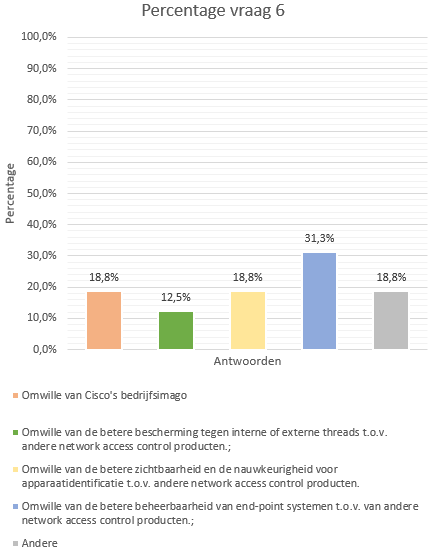
\includegraphics[width=0.50\textwidth]{Vraag6.png}
	\caption{Grafiek vraag 6}
	\label{fig:graf6}
\end{figure}
Uit vraag 7 kan afgeleidt worden dat 'Identiteits- en toegangsbeer','beleidshandhaving', 'Functionaliteit' en 'Uitbreidbaarheid' de belangrijke kermerken voor de keuze van het type network access control. Figuur \ref{fig:vraag7} toont daarbij de resultaten terug waarbij zeer duidelijk te zien is dat de vorige benoemde resultaten een zeer belangrijke rol spelen in de keuze van het network access control product. 

\begin{figure}[H]
	\centering
	\includegraphics[height=0.30\textheight]{Vraag7.png}
	\caption{Grafiek vraag 7}
	\label{fig:vraag7}
\end{figure}

Voor de volgende vraag kan men concluderen dat de veranderingen die bedrijven ondervinden na implementatie van Cisco Identity Services Engine dat die verschillende is van responder tot responder. Globaal gezien komt dit wel wat overeen met elkaar dat Cisco Identity Services Engine de zichtbaar van eind apparaten op het netwerk verhoogt. Maar een verbetering in troubleshooting is ook een van de veranderingen die de geënquêteerden ondervonden. Meer informatie over deze antwoorden is terug te vinden in bijlage \ref{tab:vraag8}. Vervolgens vindt 54.5\% van de geënquêteerden dat Cisco Identity Services Engine het product gelijkaardig vindt ten opzichte van andere network access control. Het is echter zo dat 9.1\% van de responders vindt dat Cisco Identity Services Engine slechter is dan zijn concurrenten. De rede achter dit is helaas onbeantwoord. Verder bevat 36.4\% van de antwoorden het antwoord 'Beter'. Figuur \ref{fig:vraag9} geeft deze verwoording visueel weer. 

\begin{figure}[H]
	\centering
	\includegraphics[height=0.30\textheight]{Vraag9.png}
	\caption{Grafiek vraag 9}
	\label{fig:vraag9}
\end{figure}

De resultaten van de vraag: 'Wat zijn volgens u de meeste voorkomende modules of use cases van Cisco Identity Services Engine?' zijn in figuur \label{fig:vraag10} terug te vinden. Hier is duidelijk te zien dat merendeel van de geënquêteerden vindt 'Identity-based network access control' de belangrijkste use case van Cisco Identity Services Engine. Vervolgens komt het 'Policy-based network access control' dat gevolgd wordt door het 'Thread-Centric network access control'. Hieruit kan men concluderen dat de proef een onderzoek uitvoert naar de bijna bijna belangrijkste use cases. Het is toch verbazend dat slecht 7.7\% van de personen koos voor een 'Port-based network access control' use case. 

\begin{figure}[H]
	\centering
	\includegraphics[height=0.30\textheight]{Vraag10.png}
	\caption{Grafiek vraag 10}
\end{figure}

Daarnaast blijkt ook dat 54.5\% zegt dat Cisco Identity Services Engine nadelen kent binnen een netwerk. Deze nadelen uiten zich als 'Certificate updates require nac to shut down', 'het netwerk is afhankelijk van de nac oplossing', 'Instabiliteit van connecties met sommige systemen', enz. Alle antwoorden zijn terug te vinden in bijlage \ref{tab:vraag13}. Verder werd er ook heel wat voordelen opgesomd door de vakspecalisten die weergegeven zijn in \ref{tab:vraag11}.
\newline
\newline
Uit vragen 14 en 15 is gebleken dat Cisco Identity Services Engine een logische keuze is ten opzichte van andere network access control producten. De resultaten van vraag 14 is 90.9\% voor het antwoord 'Ja' en 9.1\% met het antwoord 'Neen'. Vraag 15 toont aan dat 100\% van de vakspecalisten vindt dat een network access control product noodzakelijk is in een bedrijfsomgeving. Hieruit kan men concluderen dat een network access control zoals Cisco Identity Services Engine voor velen een echte must is.
antwoorden zijn terug te vinden in bijlage \ref{tab:vraag13}. Verder werd er ook heel wat voordelen opgesomd door de vakspecalisten die weergegeven zijn in \ref{tab:vraag11}.
\newline
\newline
18.2\% van de personen die de enquête invulden vinden dat er functionaliteiten ontbreken in Cisco Identity Services Engine. De betreffende missende functionaliteiten zijn 'Industriële gerichtheid, incl. goede support voor staticshe ip adressen.' en 'Saml integratie in een samenwerking met Azure AD en Captive portal voor byod.".


Tot slot kreeg Cisco Identity Services Engine een gemiddelde beoordeling van 3.91 op 5 waarbij 90.9\% van de geënquêteerden dit product zou aanbevelen aan anderen.





